\section{Bevor es losgehen kann - PC und Smartphone einrichten}
Bevor es mit der eigentlichen Programmierarbeit losgehen kann, muss zuerst das schon erw\"ahnte Android \ac{SDK}, von der Google-Developer-Seite \footnote{\url{http://developer.android.com/sdk/index.html}} heruntergeladen und installiert werden. Ist dies erledigt, kann es eigentlich schon fast losgehen.

\subsection{Der Android SDK Manager} \label{Der Android SDK Manager}
Bevor die Programmierarbeit losgehen kann muss nach der installation zuerst der "`Android SDK Manager"' gestartet werden. Dies ist zum einen wichtig, um die neusten Updates zu laden, aber auch um die passenden APIs welche Verwendung finden sollen zu bekommen.

Wie schon erw�hnt, ist der Manager zum einen die Update-Plattform des \ac{SDK}-Packets und zum anderen auch der Installer f�r neue Packete.

Beim starten des \ac{SDK} Managers werden Updates f�r schon installierte Packete angeboten. Damit der Download und die Installation startet, muss der Nutzer diesen Vorgang best�tigen. Sind alle Updates geladen und werden keine neuen Packete ben�tigt kann der Manager wieder geschlossen werden.

Beim ersten Starten des Managers muss ausgew�hlt werden auf welchem API-Level (welcher Android-Version) programmiert werden soll. Da Android relativ weit abw�rtskompatibel ist, empfiehlt es sich bei einem neuen Projekt immer die neuste API zu installieren. 

Durch die Verwendung der neusten API ist zum einen garantiert, dass das Projekt auf der neusten Android-Version l\"auft, zum anderen ist sichergestellt, dass das Projekt relativ lange ohne \"Anderungen mit zuk\"unftigen Versionen lauff\"ahig bleibt.

Wurde eine API geladen kann die \ac{IDE} ge\"offnet und mit dem Programmieren begonnen werden.

\subsection{Die Eclipse \ac{IDE} mit dem \ac{ADT} Plugin}
Falls bei ersten Start unter Ubuntu der Fehler: \texttt{error while loading shared libraries: \\libstdc++.so.6: cannot open shared object file: No such file or directory}

Damit das \ac{ADT}-Plugin unter Ubuntu eigesetzt werden kann, m\"ussen drei zus\"atzliche Bibliotheken nachgeladen werden. Dies ist zum Beispiel mit dem folgendne Konsolenbefehl m\"oglich.
\lstinputlisting{Code/libInstall.sh}

Im Bild \ref{Eclipse_IDE} ist ein Screenshut der Eclipse \ac{IDE} mit dem installierten \ac{ADT}-Plugin zu sehen, wie es nach der Installation vom \ac{SDK} aussehen sollte.

Im oberen Teil ist die Steuerleite zu finden, \"uber deren Butten zum Beispiel ein Debug durchgef\"uhrt oder das Projekt gestartet werden kann. Hier sind auch Button zum starten des \ac{SDK}-Managers oder die Virtual-Device-Auswahl zu finden.

Im linken Abschintt des Fensters ist der in Eclipse \"ubliche Projektbaum (Projektexplorer) zu finden, welcher die vorhandenen Projekte anzeigt. Im Bild handelt es sich hier um zwei Projekte, welche im Abschnitt \ref{Ein Projekt Anlegen} genauer geschrieben werden. 

Im mittleren Teilfenster, der IDE, ist der eigentliche Editor f\"ur den Quellcode zu sehen. In der Abbildung \ref{Eclipse_IDE} ist die Projektbau markierte Datei, im Editor, zu sehen.

Der rechte Teil des Fensters stellt die im Editor angezeigte Klasse schematisch dar. Hier sind unter dem Klassennamen alle Methoden und klassenweite Instanzen zu sehen. \"Uber einen Klick auf ein Element springt der Editor zur gew\"ahlten Methode beziehungsweise Variable.

Im unteren Bereich ist zum einen die Problem-Ansicht von Eclipse, die Console und die "`Logcat"' zu finden. Bei der Logcat handelt es sich um eine Debuganzeige, welche Warnungen, Fehler und Informationen im Android-Betriebssystem anzeigt. Wie Logcat zu benutzen ist und wie eine Anzeige innerhalb einer App generiert wird, wird im Kapitel ????? genauer beschrieben.

\begin{figure}[!ht]
\centering
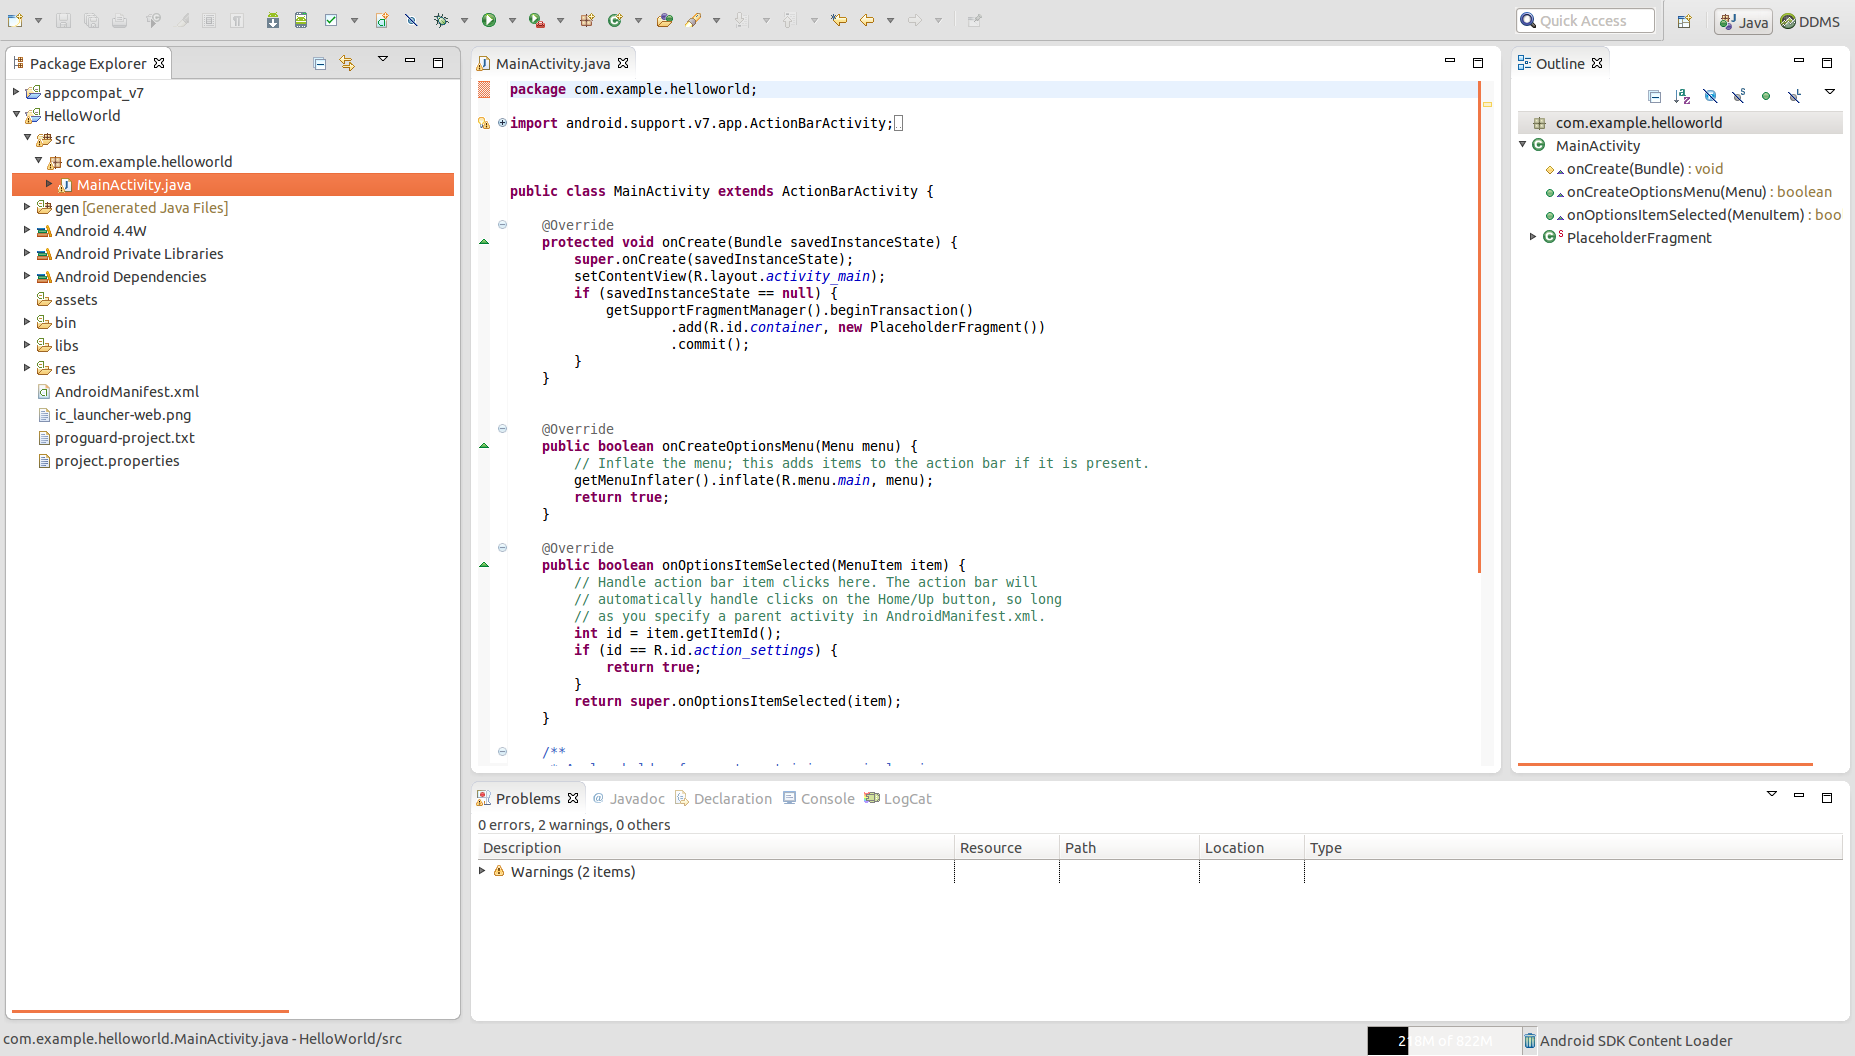
\includegraphics[width=16cm]{Bilder/IDE_Screenshut.png}
\caption{Die Eclipse \ac{IDE} mit dem \ac{ADT}-Plugin}
\label{Eclipse_IDE}
\centering
\end{figure}

\subsubsection{Ein Projekt Anlegen} \label{Ein Projekt Anlegen}
Um eine App zu programmieren wird ein Projekt ben\"otigt, welches mittles eines Rechtsklicks in den Projektexplorer geschieht. Nun muss f\"ur ein neues Projekt "`Android Application Project"' gew\"ahlt werden. \"Uber den somit aufgerufenen Wizard ist es m\"oglich die grundlegende Projektstrucktur zu erstellen. 

Wird dem Wizard in der standardkonfiguration gefolgt, wird eine "`Hello World"' App erstellt, welche den Text "`Hello World"' am Bildschirm ausgibt. \cite{Kuehn12}

Nach dem Anlegen sind zwei Projekte im Verzeichnis zu finden. Zum einen das "`HelloWorld"'-Projekt, welches die App enth\"alt und zum anderen ein Projekt mit dem Namen "`appcmpat\_v7"', welches die f\"ur ein Projekt ben\"otigten Libarys enth\"alt. Das HelloWorld-Projekt verweist auf die, automatisch erstellten, Projekt-Libarys von appcompat\_v7.

\"Uber die Schaltfl\"ache, mit dem Play-Symbol, in der oberen IDE-Leiste kann die App gestart werden.
\newpage

\subsubsection{Die App im Virtual Device Ausf\"uhren}
\begin{wrapfigure}{r}{4,95cm}
\vspace{-13pt}
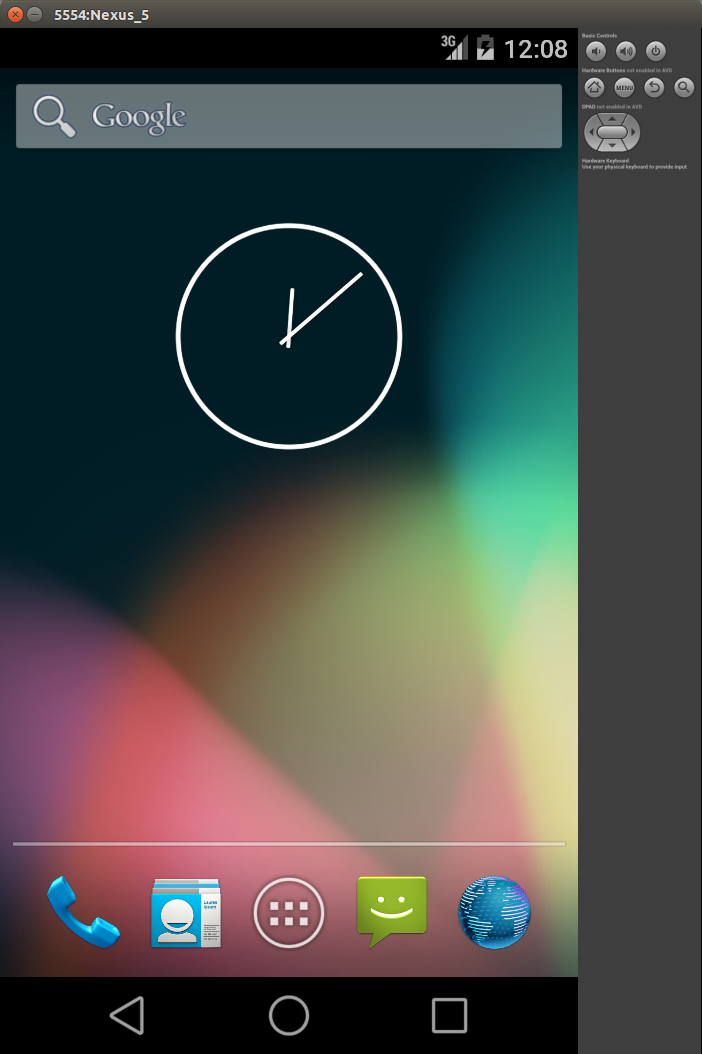
\includegraphics[width=4.95cm]{Bilder/VirtualDeviceScreenShot.png}
\caption{Android L Startbildschirm des Virtual Device}
\label{Startbildschirm des Virtual Device}
\vspace{-50pt}
\end{wrapfigure}

Nach dem Starten der App muss eine Auswahl getroffen werden, auf welchem Ger\"at die App installiert und gestartet werden soll.

Hierf\"ur muss einmalig ein Virtaul Device mit der gew\"unschtem Betriebssystem-Version erstellt werden. Au\ss{}erdem besteht die M\"oglichkeit reale Ger\"ate, wie ein Nexus 5 nicht nur in der Prozessor- und Arbeitsspeicherleistung zu simulieren sondern auch die Bildschirmgr\"o\ss{}e und Aufl\"osung.

Wurde ein Virtual Device gew\"ahlt, wird die Virtualisierung des Ger\"ates gestartet.

\subsubsection{Die App auf realer Hardware Ausf\"uhren}
Um eine App auf einem realen Androidger\"at ausf\"uhren zu k\"onnen, muss in diesem die Entwickleroption freigeschaltet werden. Dies geschieht im Hauptmen\"u unter Einstellungen. Im Men\"upunkt "`\"Uber das Telefon"' muss sieben mal auf die Build-Nummer getippt werden um die Entwickleroptionen freizuschalten.

Ist das geschehen, ist im Einstellungsmen\"u unter System der Eintrag "`Entwickleroptionen"' sichtbar. Hier k\"onnen nun viele f\"ur die Entwicklung wichtige Einstellungen vorgenommen werden. \cite{EntwickleroptionenFreischalten}

Um eine App von der IDE aus auf ein Ger\"at zu \"ubertragen muss der Eintrag "`USB-Debugging"' unter Entwickleroptionen aktiviert werden. Ist dies geschehen, muss das Ger\"at per USB-Kabel an den Entwicklungsrechner mit der IDE angeschlossen werden. 

Ist das Ger\"at angeschlossen fordert es eine Best\"atigung um App's, von dieser Quelle, installieren zu k\"onnen.

Wird nun die Play-Schaltfl\"ache bet\"atigt, fragt die IDE ob es die App auf dem realen Ger\"at oder im Virtual Device starten soll.


